% Bloques de figura listos para pegar en el articulo.
%
% Los PDF salen ya con el tamano exacto de columna (3.45 in) o de pagina
% (7.16 in), asi que se incluyen SIN escalar: un \includegraphics[width=...]
% estiraria tambien la tipografia de la figura y los 8 pt dejarian de serlo.
%
% En el preambulo:
%   \usepackage{graphicx}
%   \graphicspath{{figures_py/}}

% ======================================================================== 1
\begin{figure*}[!t]
  \centering
  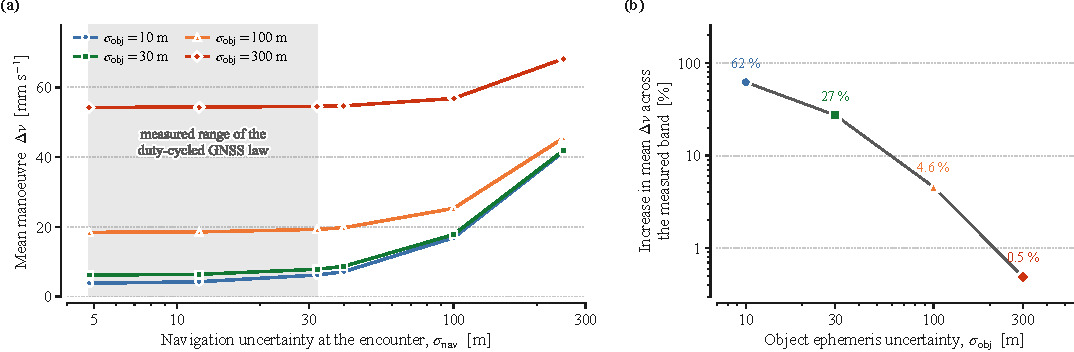
\includegraphics{fig01_coupling}
  \caption{Coupling between navigation quality and manoeuvre cost is
  conditional on the object's ephemeris. (a)~Median tangential impulse over
  $1500$ sampled conjunction geometries against the navigation uncertainty at
  the encounter, one curve per object ephemeris uncertainty
  $\sigma_{\mathrm{obj}}$; the shaded band is the range spanned by the measured
  duty-cycled GNSS law of Fig.~\ref{fig:nav} ($4.8$--$32.1$\,m). (b)~The same
  data read as a sensitivity: the increase in median $\Delta v$ across that
  band. Tightening the navigation only buys something when the object is known
  better than the band itself, $+3254\,\%$ at $\sigma_{\mathrm{obj}} = 10$\,m
  against $+0.5\,\%$ at $300$\,m.}
  \label{fig:coupling}
\end{figure*}

% ======================================================================== 2
\begin{figure}[!t]
  \centering
  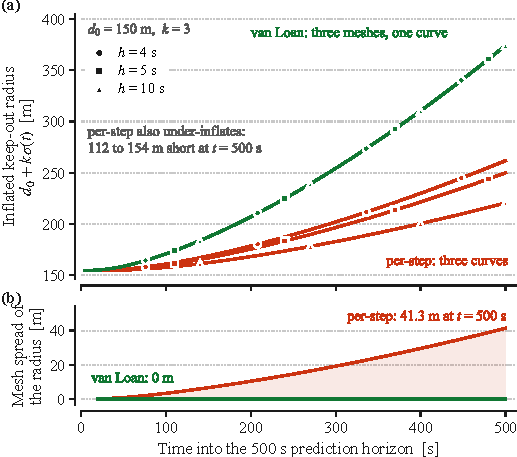
\includegraphics{fig02_koz_consistency}
  \caption{The inflated keep-out radius must be a function of time, not of the
  prediction mesh. (a)~$d_0 + k\sigma(t)$ over a $500$\,s horizon split three
  ways. Adding a fixed per-step process-noise increment makes the radius depend
  on the splitting; discretising the continuous process-noise power spectral
  density over the step with the van Loan method collapses the three onto one
  curve. (b)~The spread across the three meshes, which reaches $41.3$\,m at
  $t = 500$\,s for the per-step scheme and is zero, to the stored precision, for
  van Loan.}
  \label{fig:koz}
\end{figure}

% ======================================================================== 3
\begin{figure*}[!t]
  \centering
  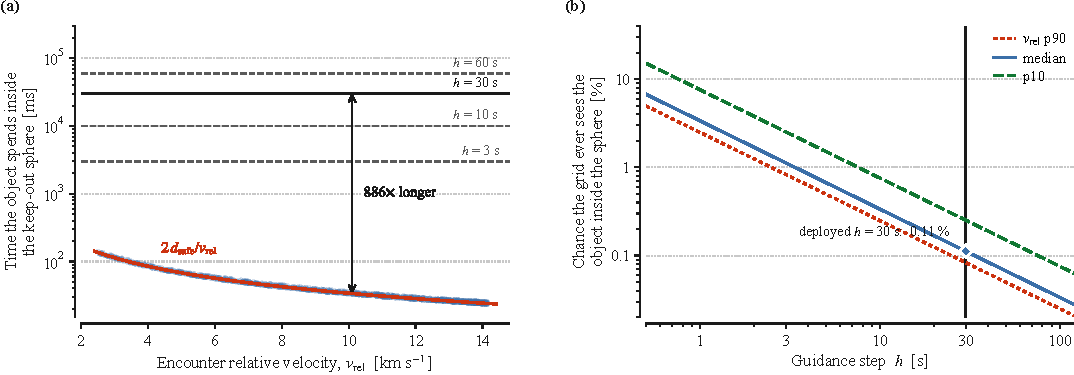
\includegraphics{fig03_architecture_cost}
  \caption{Enforcing the collision constraint inside the QP does not close in
  real time; planning the manoeuvre outside it does. (a)~Solve-time
  distribution per configuration, with each configuration's own deadline
  dashed. The median is not the problem: up to $14.9\,\%$ of solves overrun
  their guidance step and the worst cases reach $45$ and $77$\,s. (b)~The same
  data as empirical distributions of solve time normalised by each
  configuration's deadline. The proposed architecture solves in $2.8$\,ms
  median and $62$\,ms worst against a $30$\,s deadline. Sample sizes are $41$
  to $134$ solves for the QP-internal cases, so the extreme quantiles rest on
  one or two solves each.}
  \label{fig:timing}
\end{figure*}

% ======================================================================== 4
\begin{figure}[!t]
  \centering
  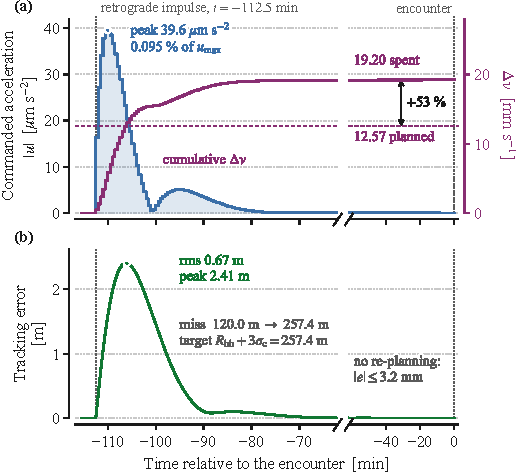
\includegraphics{fig04_execution}
  \caption{One encounter executed end to end: an $88.15^\circ$ plane crossing at
  $10.0$\,km/s. (a)~Commanded acceleration and cumulative $\Delta v$. The
  guidance layer plans a single retrograde tangential impulse of $12.6$\,mm/s at
  $-112.5$\,min and the MPC tracks the retargeted reference, spending
  $19.2$\,mm/s to deliver it: a $53\,\%$ overhead for following a continuous
  reference instead of firing an impulse. The peak command is $39.6\,\mu$m/s$^2$,
  $0.095\,\%$ of the $1$\,N authority. (b)~Tracking error, $0.67$\,m rms and
  $2.41$\,m peak. The miss distance opens from $120.0$\,m to $257.4$\,m against
  a required $R_{\mathrm{hb}} + 3\sigma_c = 257.4$\,m; the plan is not revisited
  after the burn.}
  \label{fig:exec}
\end{figure}

% ======================================================================== 5
\begin{figure}[!t]
  \centering
  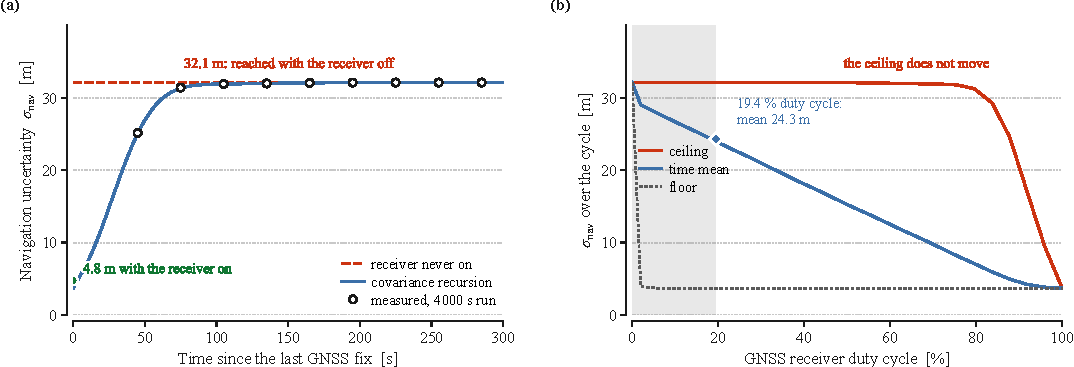
\includegraphics{fig05_navigation}
  \caption{Measured cost of duty-cycling the GNSS receiver. (a)~A $900$\,s
  window of the $4000$\,s record, with the receiver on $19.45\,\%$ of the time.
  (b)~The same record collapsed onto time since the last fix: the position
  uncertainty leaves $4.8$\,m, saturates at $32.1$\,m and is within $1\,\%$ of
  that level after $89$\,s, whatever the length of the gap. The cost of
  duty-cycling is therefore bounded, and $32.1$\,m is the value that reaches the
  guidance layer.}
  \label{fig:nav}
\end{figure}

% ======================================================================== 6
\begin{figure}[!t]
  \centering
  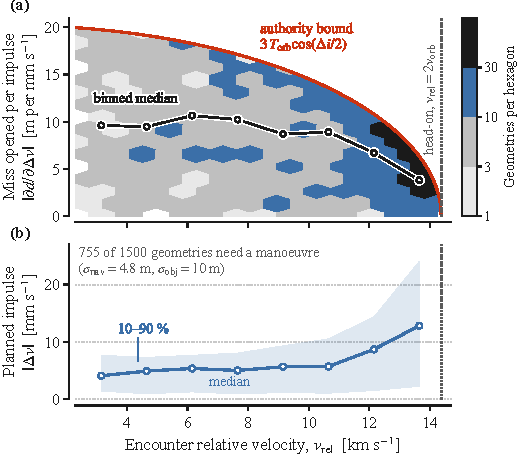
\includegraphics{fig06_tangential_authority}
  \caption{A single tangential impulse loses its authority in a head-on
  encounter. (a)~Miss distance opened per unit impulse over the $1500$
  geometries, against the encounter relative velocity, with the analytic
  envelope $3\,T_{\mathrm{orb}}\cos(\Delta i/2)$. The envelope closes as
  $v_{\mathrm{rel}} \rightarrow 2v_{\mathrm{orb}}$, so no amount of $\Delta v$
  opens the miss. (b)~The impulse the planner asks for, median and $10$--$90\,\%$
  band, rising by a factor of $3.1$ from the slowest to the fastest encounters.
  Colour in~(a) is a raw case count and the study samples $\Delta i$ uniformly,
  so part of the left-to-right gradient is the sampling and not the physics.}
  \label{fig:authority}
\end{figure}

% ======================================================================== 7
\begin{figure*}[!t]
  \centering
  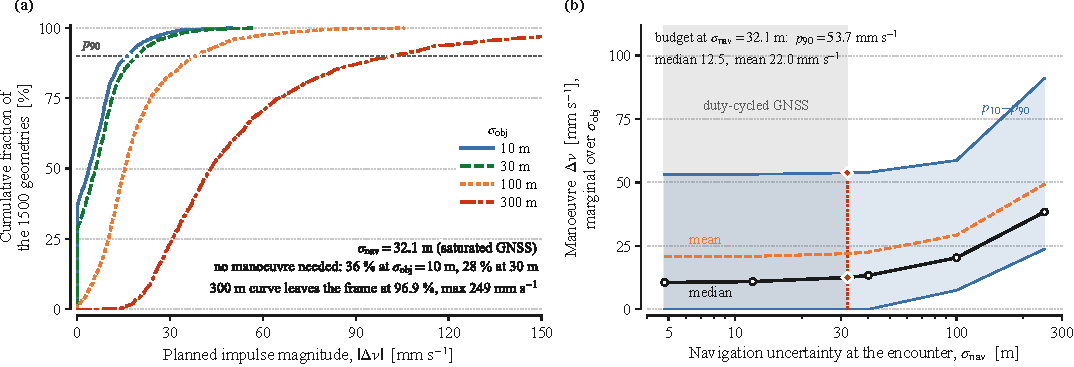
\includegraphics{fig07_dv_distribution}
  \caption{The $\Delta v$ budget is a tail, not a median. (a)~Empirical
  distribution of the planned impulse at the measured operating point
  ($\sigma_{\mathrm{nav}} = 32.1$\,m), one curve per object ephemeris quality;
  the ordinate at $|\Delta v| = 0$ is the fraction of geometries already safe
  without manoeuvring. (b)~Median and $10$--$90\,\%$ band against navigation
  uncertainty, marginalised over ephemeris quality with a uniform weight on the
  four simulated levels. At the operating point the median is $12.5$\,mm/s and
  the $90$th percentile $53.7$\,mm/s, which is the number a tank has to be sized
  against. Values are per encounter; the study carries no conjunction rate.}
  \label{fig:budget}
\end{figure*}

% ======================================================================== 8
\begin{figure}[!t]
  \centering
  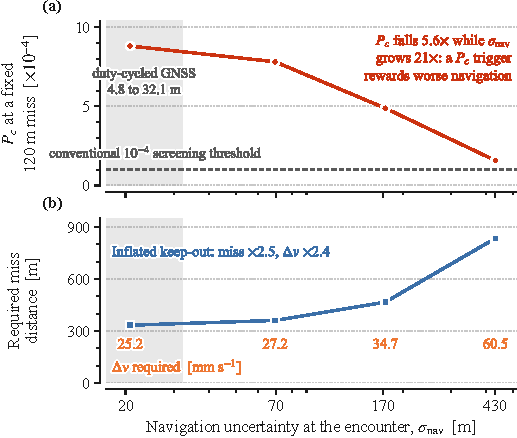
\includegraphics{fig08_probability_dilution}
  \caption{Why the design constrains a distance and not a collision
  probability. (a)~With the miss distance held at $120$\,m, the collision
  probability computed with the Foster formulation \emph{falls} from
  $8.8\times10^{-4}$ to $1.6\times10^{-4}$ as the navigation uncertainty grows
  by a factor of $21$: a larger covariance spreads the same probability mass
  over a larger area. A guidance law triggered on a $P_c$ threshold would
  therefore reward worse navigation. (b)~The covariance-inflated keep-out
  distance instead grows monotonically, $333 \rightarrow 835$\,m, and with it
  the required impulse, $25.2 \rightarrow 60.5$\,mm/s. This sweep is the
  standalone conjunction demonstrator, with its own object-covariance
  assumption of $\sigma_{\mathrm{obj}} = 150$\,m.}
  \label{fig:dilution}
\end{figure}
